\documentclass[a4paper, 12pt]{article}
\usepackage{a4wide}
\usepackage{textcomp}
\usepackage{listings}
\usepackage{color}

\usepackage{graphicx}
\graphicspath{ {./images/} }

\usepackage[backend=biber,style=numeric]{biblatex}
\addbibresource{bibliography.bib}

\definecolor{dkgreen}{rgb}{0,0.6,0}
\definecolor{gray}{rgb}{0.5,0.5,0.5}
\definecolor{mauve}{rgb}{0.58,0,0.82}

\lstset{frame=tb,
  language=Java,
  aboveskip=3mm,
  belowskip=3mm,
  showstringspaces=false,
  columns=flexible,
  basicstyle={\small\ttfamily},
  numbers=none,
  numberstyle=\tiny\color{gray},
  keywordstyle=\color{blue},
  commentstyle=\color{dkgreen},
  stringstyle=\color{mauve},
  breaklines=true,
  breakatwhitespace=true,
  tabsize=3
}

\begin{document}

    \title{A Graphical Programming Language Editor}
    \author{Candidate No. 198719}
    \date{November 3, 2020}
    \clearpage\maketitle
    \thispagestyle{empty}

    \newpage\clearpage\thispagestyle{empty}
    \tableofcontents
    \newpage
    \setcounter{page}{1}

    \section{Introduction}
    Graphical programming can be a fantastic and intuitive way to introduce new programmers to
    the scene. When programmers ask others for assistance, those helping typically do so in a visual 
    style, using whiteboards, drawing flowcharts, with boxes and arrows indicating the flow 
    of the program. Why can't we make programs in the same style if we find it so helpful to read? 
    The concept behind graphical programming is specifying the elements of the program graphically 
    rather than textually~\cite{dehouck2015maturity}.

    Popular examples of graphical programming include Scratch, as well as a personal favourite that 
    I used during my GCSE Computing education, App Inventor!
    What's clever about Scratch is its simplicity due to the block-based visual programming, aimed 
    towards younger children to help them get into coding!

    \begin{figure}[h]
        \centering
        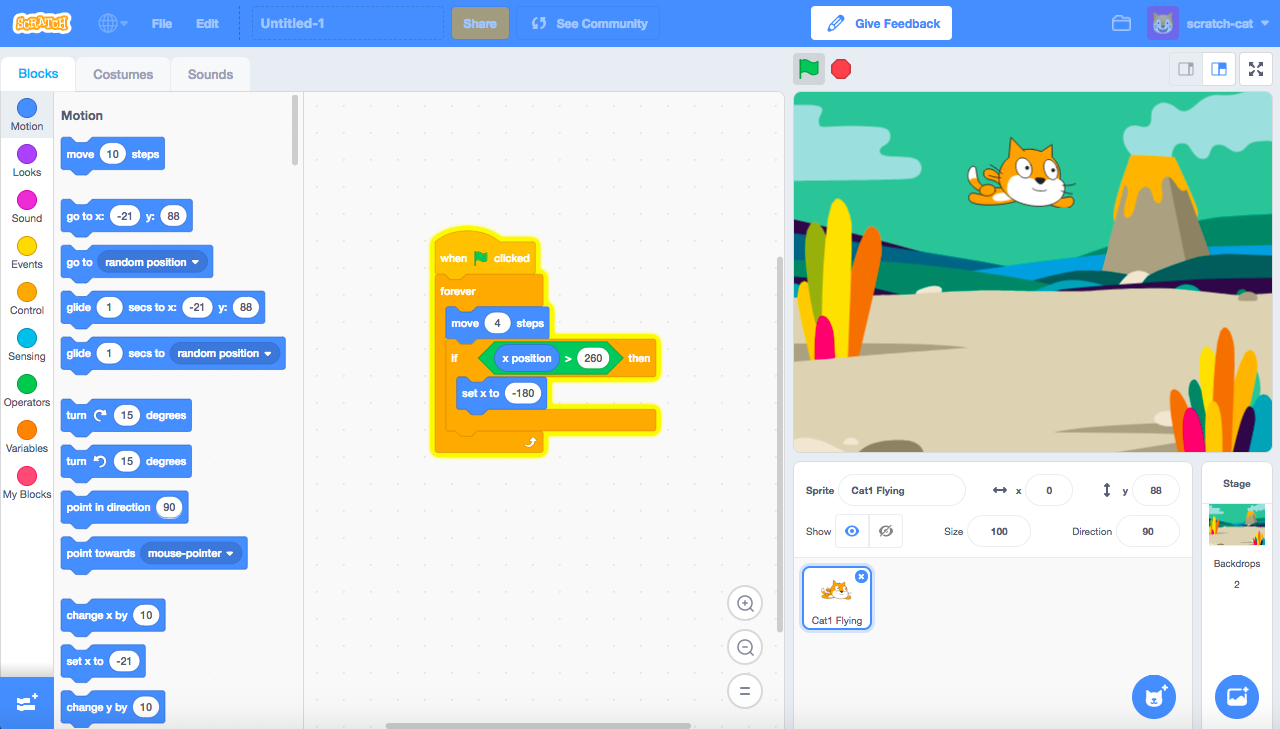
\includegraphics[width=160mm]{scratch_image}
        \caption{Scratch's visual scripting over a white canvas~\cite{thescratchteam}.}
    \end{figure}

    \clearpage
    MIT App Inventor is one of my personal favourites after experiencing it myself during GCSEs, 
    having to building an on-campus application for a University! It uses a graphical user 
    interface, similar to Scratch, as well as providing the blocks that you can use, visible on 
    the left hand side.

    \begin{figure}[h]
        \centering
        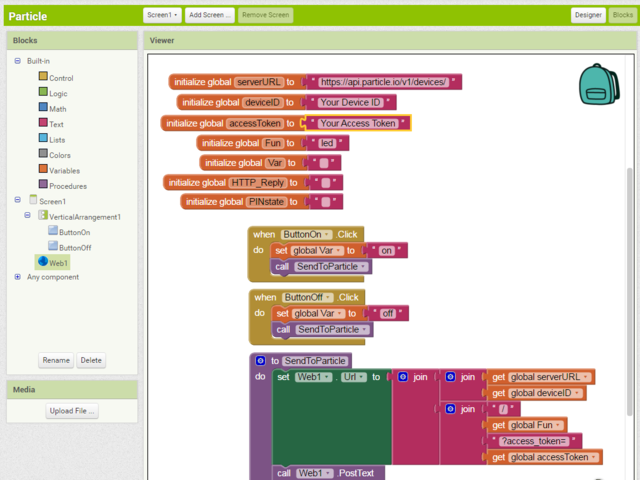
\includegraphics[width=150mm]{app_inventor}
        \caption{MIT App Inventor graphical programming~\cite{adafruit}.}
    \end{figure}

    Both what Scratch and App Inventor do superbly is colour code their blocks to identify 
    exactly what they are representing. There are colour coded blocks for variables, events 
    and controls, and so on! For instance in App Inventor, variables are coloured in Orange 
    blocks, and procedures and show in a big purple block, encapsulating all the blocks like 
    a function.

        \subsection{Aims}
            The aim of this project is to design and implement a simple interface for the
            user to graphically program basic functions. Simple functions may include:

            \begin{itemize}
                \item loops.
                \begin{itemize}
                    \item this includes \texttt{for} and \texttt{while} loops.
                \end{itemize}
                \item conditional statements, such as \texttt{if} statements.
                \item implementing and interacting with data structures, such as lists.
                \item procedures like methods/functions.
                \item variables!
            \end{itemize}
            
            This is necessary as it provides another programming viewpoint for the user,
            which can aid them understand the process and flow of how said program may
            be running. It is also friendly and less intimidating for newer users,
            relative to a textual/command line script.
            
            I am going to program this is Java, my most experienced language, making use
            of Java's smart GUI design feature, whilst learning and building knowledge on
            said feature for my own experience.

        \subsection{Objectives}
            The main objectives are:

            \subsubsection{To investigate system requirements to produce a requirements
            specification.}

            \subsubsection{To select and justify an appropiate simple design for the
            project.}

            \subsubsection{Implement a simple interface for users which is easy to
            understand.}

            \subsubsection{Functional and working loops, conditionals and data structures
            that can be interacted with.}

        \subsection{Problem Area}
            The main challenge of implementing an interface to be able to program on is the required 
            time and skill set. This project may never be fully complete as more work can always be 
            done to improve the functionality of the interface, or making the interface more user-friendly.

            The project can be broken down into key areas that require focusing on:
        
            \begin{itemize}
                \item Graphical Design - modelling, interface, simplicity, GUI.
                \item Functionality - programming.
            \end{itemize}

            I have limited GUI design in Java from my 2nd year module, Further Programming, therefore this 
            process can be said to take up a large amount of time. Careful consideration is needed to 
            not overspend my time on the GUI design process, and rather get the functionality of said 
            interface to work.

            Functionality requires programming to be clean and efficient, so not to go back over the code 
            and forget what was written. Code must be documented and commented along the way to make sure 
            anyone who reads the code, including myself in the future, is able to understand what was 
            written and why it was decided.

            \subsection{Expected Outcomes}
            The expected outcomes of this project are a fully working, functional graphical programming 
            language interface. The user should use the tool independent from the back-end Java textual 
            code, and be able to perform the certain tasks:

            \begin{itemize}
                \item loops - create and work with basic for \& while loops.
                \item data structures - create and interact with data structures such as lists.
                \item variables - create, store data and interact with variables.
                \item procedures - create functions/methods to perform certain tasks inside them!
                \item interface - an interface for users to be able to interact with and perform the
                above outcomes.
            \end{itemize}

    \clearpage
    \section{Professional and Ethical Considerations}
        Below you will find the relevant sections of the BCS Code Conduct that apply to this 
        project. Since this project will not require any human participation, no ethical review 
        is necessary.

        \subsection{BCS Code of Conduct}
            \textbf{1.1 - have due regard for public health, privacy, security and wellbeing of others 
            and the environment;} \\\\
            This project does not feature any distressing visuals that may harm the user. \\\\
            \textbf{2.1 - only undertake to do work or provide a service that is within your professional 
            competence;} \\\\
            This project is within my professional skillset to complete. \\\\
            \textbf{2.3 - develop your professional knowledge, skills and competence on a continuing 
            basis, maintaining awareness of technological developments, procedures, and standards 
            that are relevant to your field;} \\\\
            Throughout this project I will maintain my skills, but further learn and research new ideas 
            or more experienced methods to make my skills more proficient within the field. \\\\
            \textbf{2.5 - respect and value alternative viewpoints and seek, accept and offer honest 
            criticisms of work;} \\\\
            I will accept feedback by my supervisor and others and use the criticisms to develop and 
            build upon the project further. Results of feedback will not be edited. \\\\
            \textbf{3.2 - seek to avoid any situation that may give rise to a conflict of interest 
            between you and your relevant authority;} \\\\
            Throughout the project I will be respect to my colleagues and my supervisor.

    \clearpage
    \section{Related Work}
        \subsection{Scratch}
            The key goal that Scratch sticks by is trying to introduce programming to those with no
            programming experience knowledge whatsoever. Scratch has been widely distributed to school
            systems and education organisations~\cite{maloney2010scratch}. Scratch also couldn't be any
            more clearer to use, with a heading of categories for you to choose and select the difference
            blocks that provide different functionality.

            \begin{figure}[h]
                \centering
                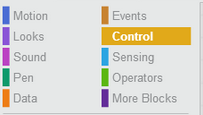
\includegraphics{scratch_blocks.png}
                \caption{Scratch's categories of blocks that you can select from.}
            \end{figure}

            The user doesn't require any documentation to understand how to use Scratch, rather they
            are able to learn on the go, hence why it is suitable to new programmers trying to get a
            basic feel of the approach and what programming can do, as well as what you are able to
            do with it!

        \subsection{MIT App Inventor}
            MIT App Inventor is another graphical programming language for building apps for Android devices.
            App Inventor is used across 195 countries, in education organisations and also self-taught
            \cite{xie2016skill}. 

            \begin{figure}[h]
                \centering
                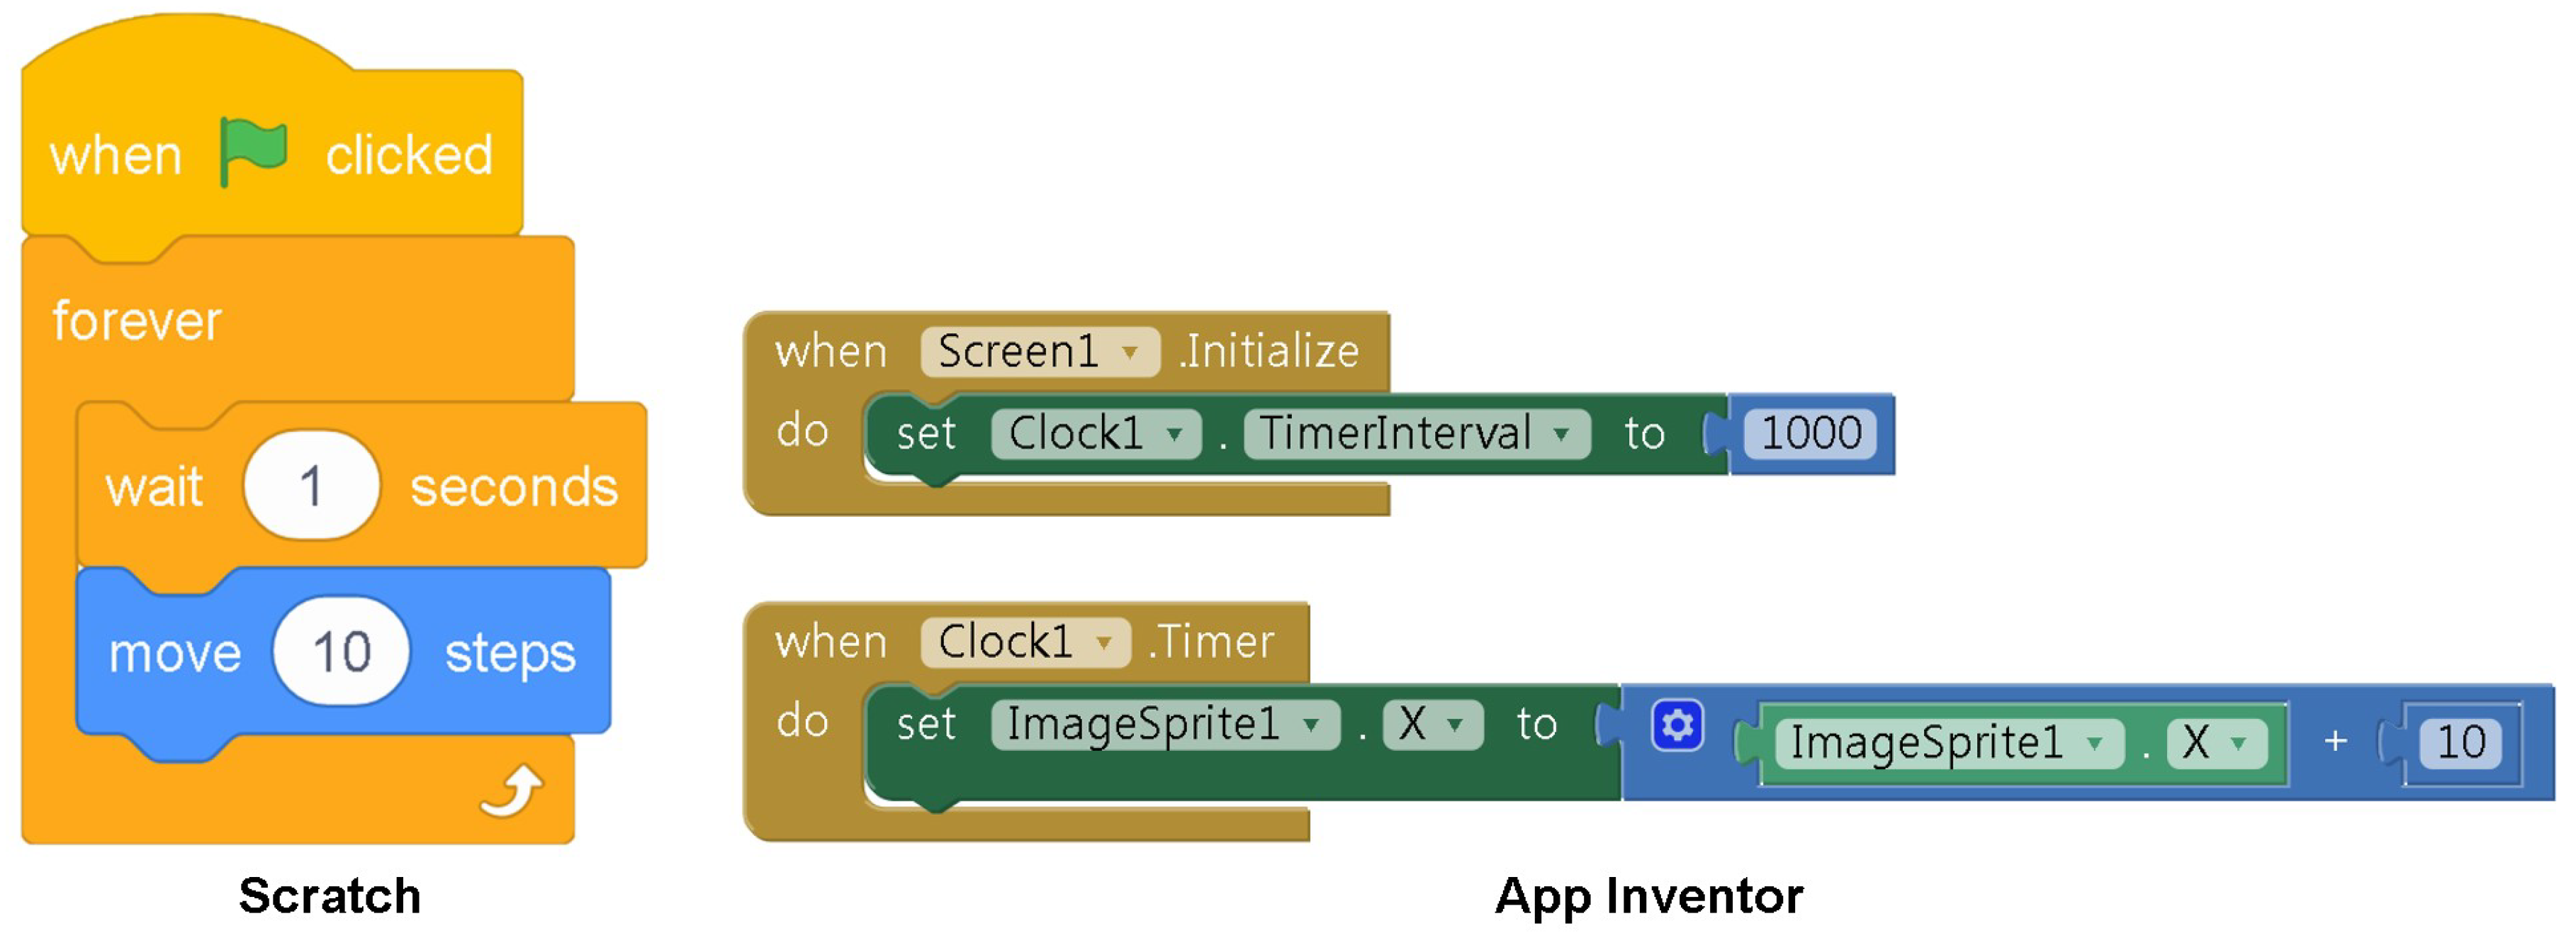
\includegraphics[width=125mm]{scratch_vs_appinventor.png}
                \caption{Graphical style of Scratch vs App Inventor~\cite{park2019comparing}. App Inventor is slightly more sophisticated.}
            \end{figure}

            \clearpage
            Scratch and MIT App Inventor are the two most widely used block-based graphical programming
            languages for students and/or pupils. As of August 2019, there were 44,981,198 registered
            users on Scratch, and 8,200,000 registered users on App Inventor~\cite{park2019comparing}.

            Both Scratch and App Inventor share the common goal of providing an educational programming
            language for new comers. Scratch is mainly used as a foundation to teach younger children
            the concepts of code, whereas App Inventor is used as the \textit{"step up"}, but both are
            used globally to make programming a bit more fun and interactive. App Inventor in particular
            is rewarding as upon running the code, an interactive mobile phone displaying your app is
            shown as the output!

        \subsection{Blockly}
            Blockly is probably by far the most modern out of the three I have proposed, and the 
            most intuitive. It's a free, web-based, open-source project by Google, built upon the 
            idea of Scratch. But what's intuitive about Blockly is the textual programming output 
            on the right-hand side of your graphical code. It can generate code in the following 
            languages~\cite{nbcbayarea}:

            \begin{itemize}
                \item Javascript.
                \item Lua.
                \item Dart.
                \item Python.
                \item PHP.
            \end{itemize}

            It can also be edited to generate code in a different textual programming language!

            \begin{figure}[h]
                \centering
                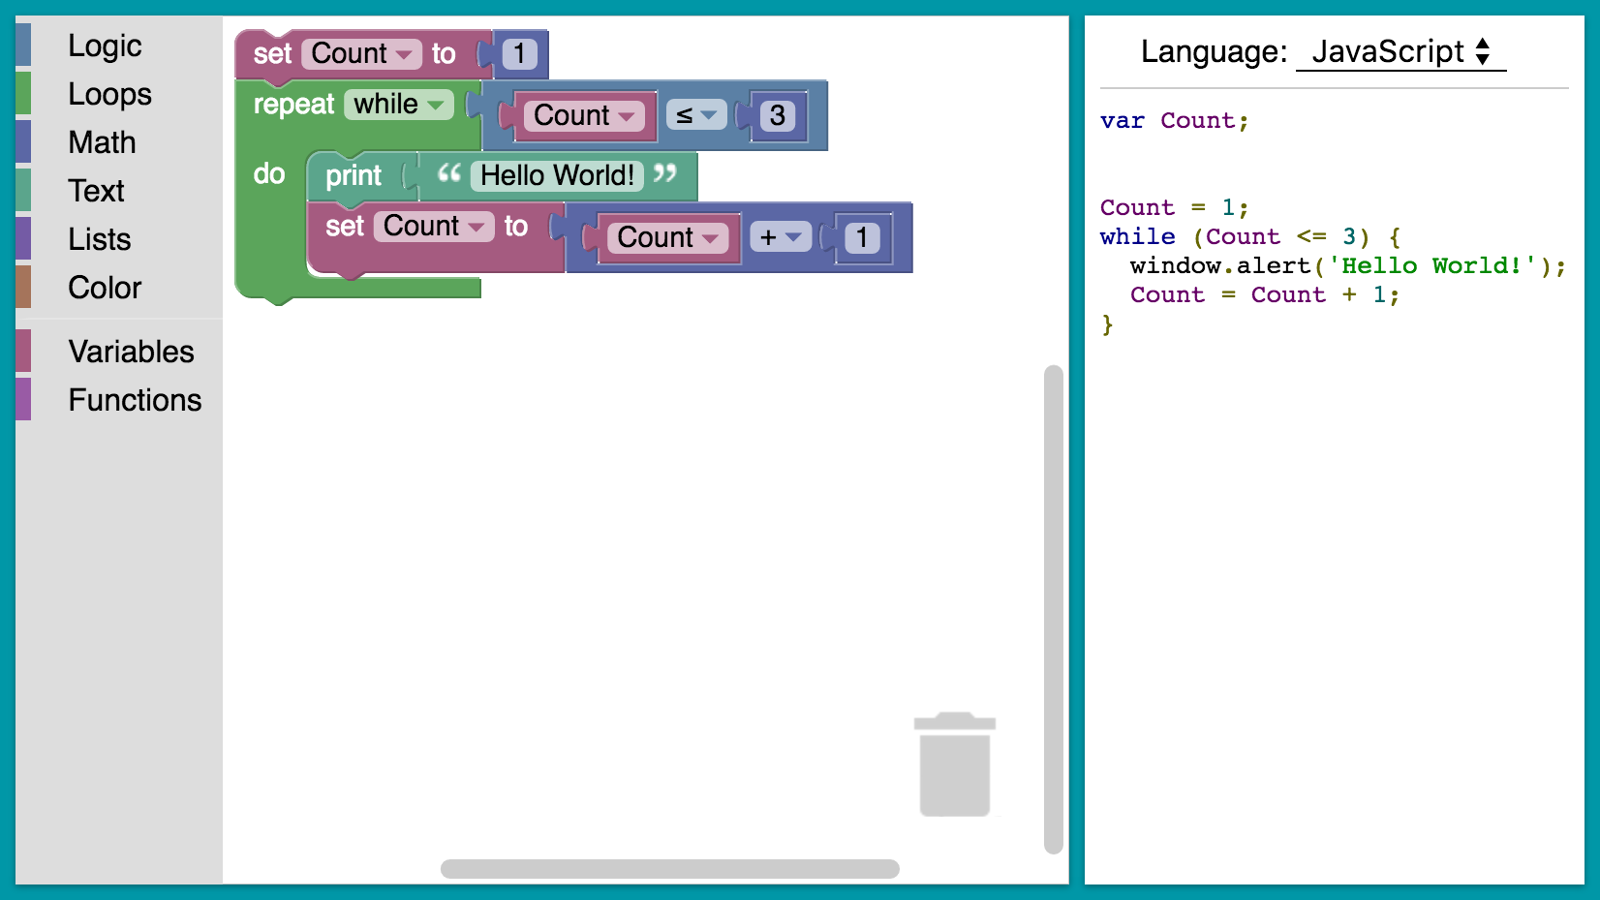
\includegraphics[width=150mm]{blockly.png}
                \caption{Blockly's modern and simple block programming design, as well 
                as the option to choose the programming language that it will syntactically 
                output as~\cite{blockly}.}
            \end{figure}

            Blockly is aimed towards new programmers to get them onboard and addicted to the visual 
            scene first. By providing the textual version of the code, perhaps this might spark a 
            passion within the user to follow through with programming. By being provided with the 
            textual code of their graphical app, they are learning and understanding what the code 
            will really look like and how they could potentially implement it themselves.

            A key part of Blockly that the developers undertook was user testing. The conditional and loop blocks were in the same category, with the same colour, 
            confusing the users who expected the program to run a certain way, when it ran differently 
            to what they were expecting ~\cite{fraser2015ten}. The developers understood this and 
            learnt from the feedback quickly, moving the conditionals to a different category, as 
            well as changing the colour too. This removed the confusion instantly. These key ways to improve 
            from feedback received is key to building a successful project.
        
        \clearpage
        \subsection{Graphical Programming}
            What all three graphical programming editors do together is follow the convention 
            of lower-case naming of variables, functions and so on that is followed in textual-based
            programming languages, for instance \textit{"if"} and \textit{"while"}. 

            \begin{figure}[h]
                \centering
                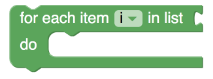
\includegraphics{lowercase_convention.png}
                \caption{The lowercase convention, as followed by Blockly as an example~\cite{pasternak2017tips}.}
            \end{figure}

            Graphical programming is not a permanent solution to programming, but rather an 
            introduction~\cite{gregoryvisual}.

    \clearpage
    \section{Requirements Analysis}
        In this section, I have taken into careful consideration the aims and objectives for this
        project. Below you will find a compiled list of software requirements, split into two
        categories: \textbf{mandatory} requirements, the fundamental requirements that is needed
        for the project to work, and \textbf{desirable} requirements, optional further requirements
        that can be met to provide further quality of life experiences for the user.

        \subsection{Mandatory Requirements}

            \begin{table}[h]
                \begin{tabular}{|l|l|}
                    \hline
                    \multicolumn{2}{|c|}{\textbf{Mandatory Requirements}}                                                                                                                                                                                                             \\ \hline
                    \textbf{Requirement}                                                                                                     & \textbf{Specification}                                                                                                                 \\ \hline
                    \begin{tabular}[c]{@{}l@{}}1. Application will work on any java-run\\ environment.\end{tabular}                          & \begin{tabular}[c]{@{}l@{}}Whether the user is on a Windows, macOS\\ or Linux system, the application will work.\end{tabular}          \\ \hline
                    \begin{tabular}[c]{@{}l@{}}2. The interface shall accept user input\\ via keyboard and mouse.\end{tabular}               & \begin{tabular}[c]{@{}l@{}}User will be able to use keyboard and mouse\\ to create and interact with the canvas.\end{tabular}          \\ \hline
                    3. The program shall run until is it killed.                                                                             & \begin{tabular}[c]{@{}l@{}}The process will not stop running until either\\ it is killed via user or forced shutdown.\end{tabular}     \\ \hline
                    \begin{tabular}[c]{@{}l@{}}4. The program will output any errors,\\ if any.\end{tabular}                                 & \begin{tabular}[c]{@{}l@{}}If there are any run-time errors, the terminal\\ will output those for the user to see.\end{tabular}        \\ \hline
                    \begin{tabular}[c]{@{}l@{}}5. The user shall be able to use functional\\ loops such as for and while loops.\end{tabular} & \begin{tabular}[c]{@{}l@{}}The user will have the ability to interact with\\ loops in the interface.\end{tabular}                      \\ \hline
                    \begin{tabular}[c]{@{}l@{}}6. The user shall be able to create\\ variables.\end{tabular}                                 & \begin{tabular}[c]{@{}l@{}}The user will be able to create and interact\\ with variables.\end{tabular}                                 \\ \hline
                    \begin{tabular}[c]{@{}l@{}}7. The user shall be able to create\\ functions or procedures.\end{tabular}                   & \begin{tabular}[c]{@{}l@{}}Users will have the ability to create functions\\ /methods that perform a variety of tasks.\end{tabular}    \\ \hline
                    \begin{tabular}[c]{@{}l@{}}8. The user will be able to create data\\ structures.\end{tabular}                            & \begin{tabular}[c]{@{}l@{}}Data structures such as lists will be available\\ for the user to implement and interact with.\end{tabular} \\ \hline
                    9. A run button.                                                                                                         & A button to run to be able to run their program.                                                                                       \\ \hline
                \end{tabular}
            \end{table}

        \clearpage
        \subsection{Desirable Requirements}
            \begin{table}[h]
                \begin{tabular}{|l|l|}
                    \hline
                    \multicolumn{2}{|c|}{\textbf{Desirable Requirements}}                                                                                                                                                                                                                                                                           \\ \hline
                    \textbf{Requirement}                                                   & \textbf{Specification}                                                                                                                                                                                                                                 \\ \hline
                    1. Colour coded blocks.                                                & \begin{tabular}[c]{@{}l@{}}The designs can be colour coded to visually\\ aid the user what they represent. For instance,\\ orange blocks for variables.\end{tabular}                                                                                   \\ \hline
                    2. Interactive sound design.                                           & \begin{tabular}[c]{@{}l@{}}A potential sound that can be producing by\\ interacting with the program. For instance,\\ dragging and dropping, clicking, etc...\end{tabular}                                                                             \\ \hline
                    \begin{tabular}[c]{@{}l@{}}3. Highlight when mouse\\ over\end{tabular} & \begin{tabular}[c]{@{}l@{}}When the mouse is hovered over an object,\\ said object could be highlighted by a glowing\\ fade, or perhaps an outline of the object.\end{tabular}                                                                         \\ \hline
                    4. Recycling bin.                                                      & \begin{tabular}[c]{@{}l@{}}A recycling bin in the bottom corner to show\\ users where they can drag and drop blocks\\ that are not needed. This could only be visible\\ when an object is being dragged, or it could always\\ be visible.\end{tabular} \\ \hline
                    5. Undo button.                                                        & A button to undo an action.                                                                                                                                                                                                                            \\ \hline
                    6. Redo button.                                                        & A button to redo an action if undone.                                                                                                                                                                                                                  \\ \hline
                \end{tabular}
            \end{table}

        My aim is to attempt to achieve all the mandatory requirements as they are underlying
        foundations of the program. All the requirements work together to build the program. 
        Without any of these requirements, this will fail to work effectively. The desirable 
        requirements that I would like to be able to implement include the undo + redo button, 
        as well as the recycling bin! Thinking about the user's goals here, these would be 
        incredibly impactful towards benefiting their quality of life experience. Having the 
        ability to undo/redo any mistakes you make, as well as simply drag and drop to the bin 
        to delete unnecessary content, only makes the lives of the user easier.

    \clearpage
    \section{Project Plan}

        \begin{figure}[h]
            \centering
            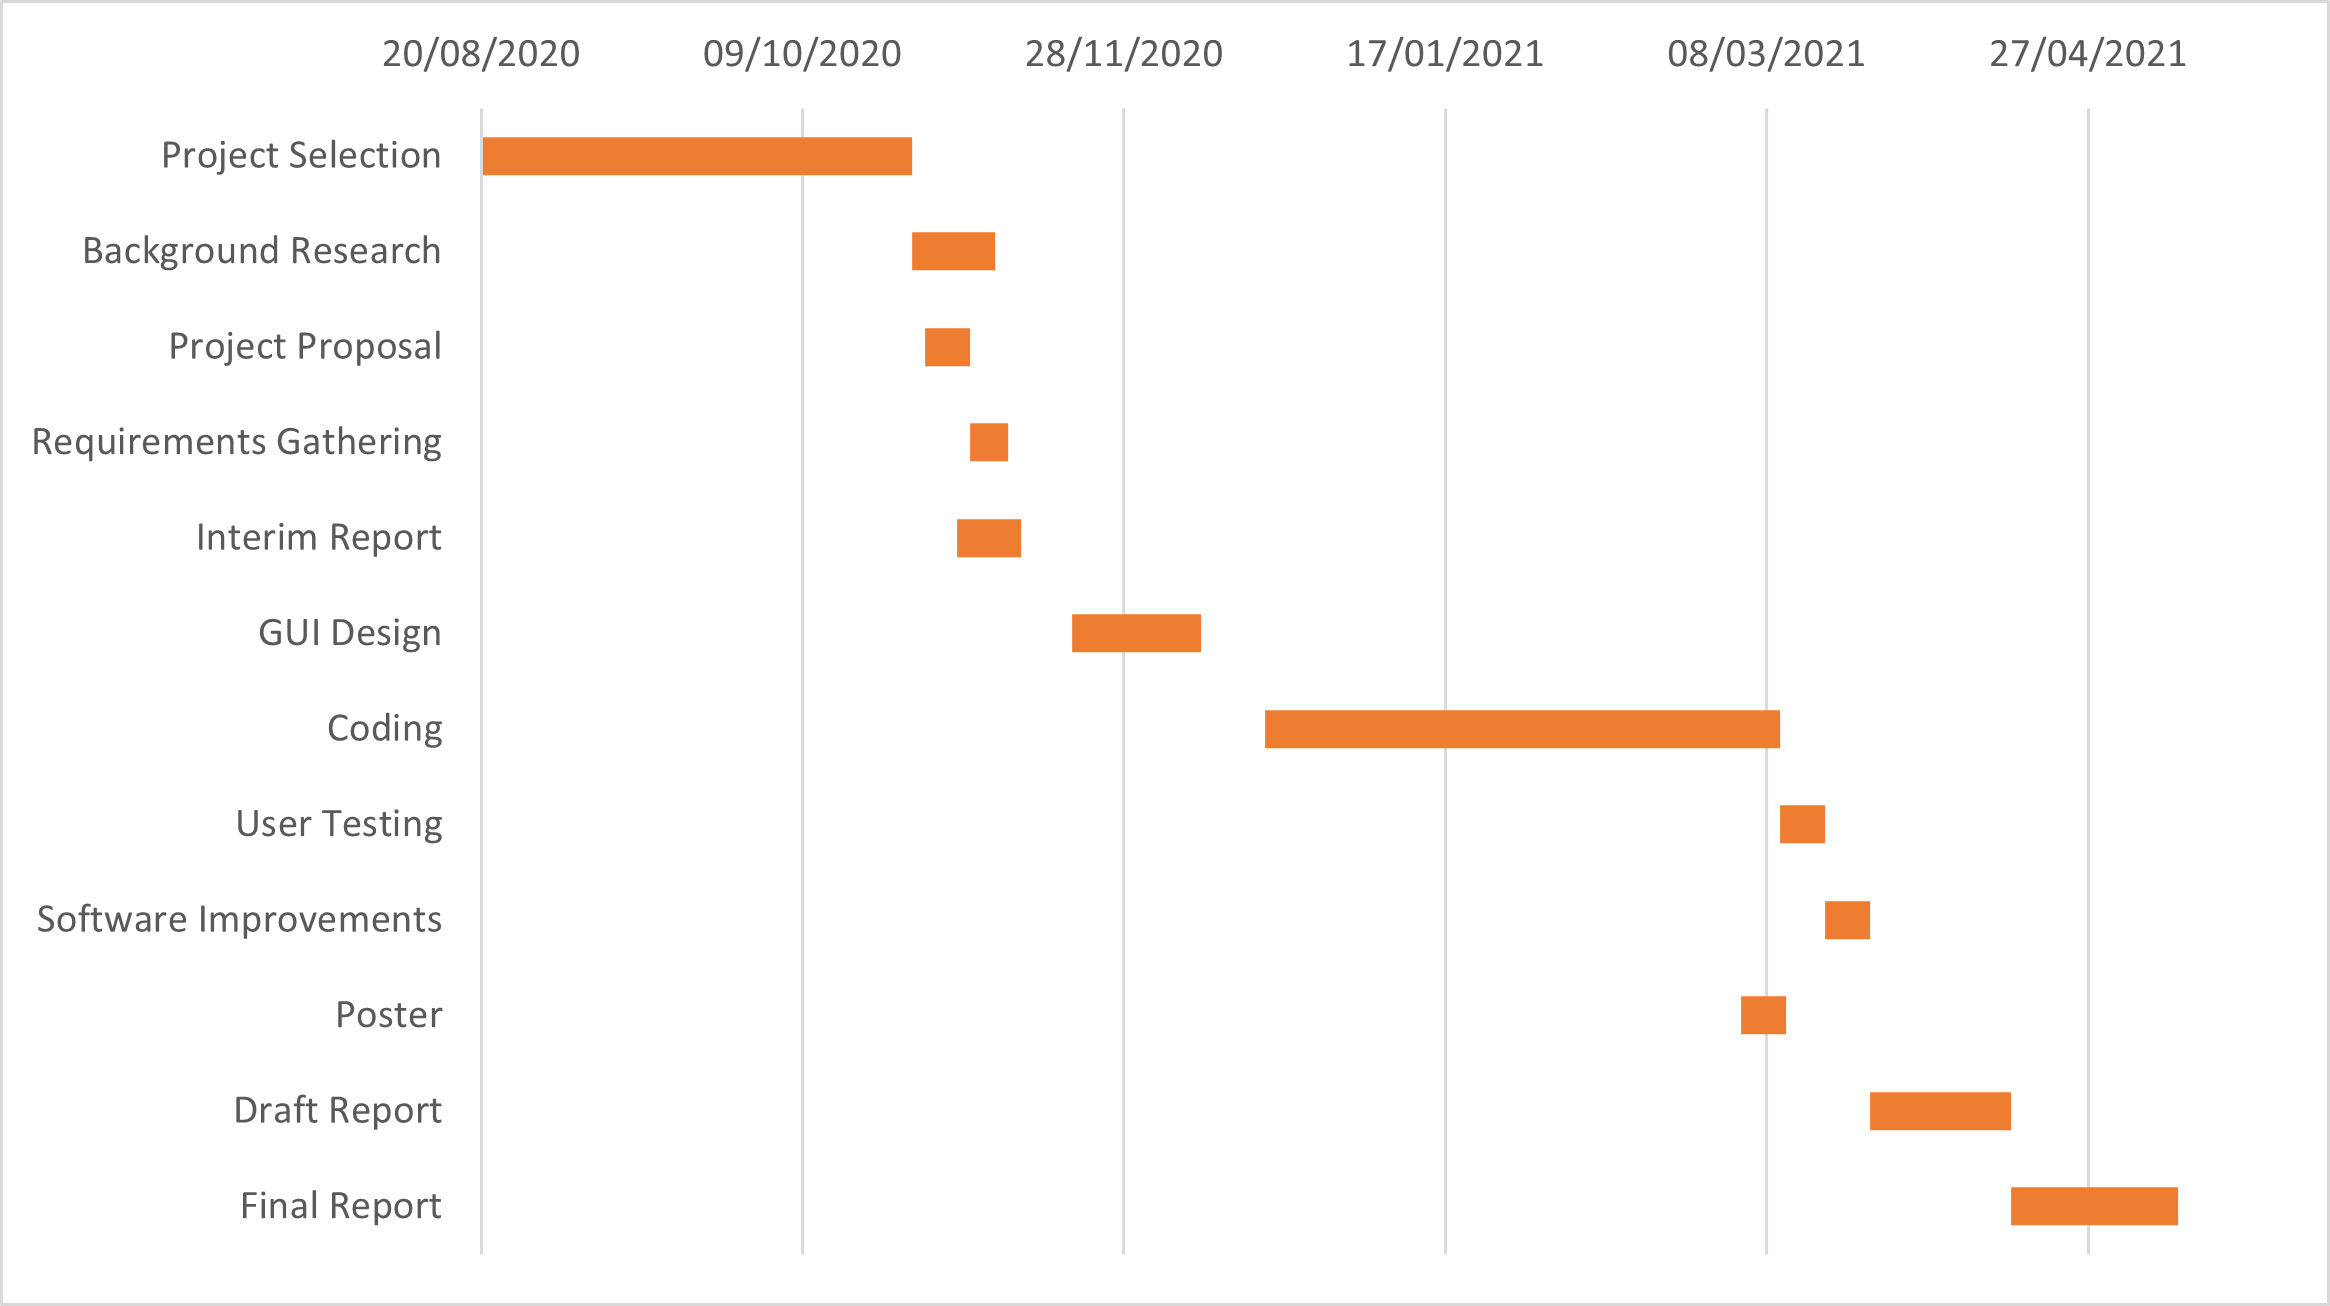
\includegraphics[width=150mm]{gantt_chart.png}
            \caption{My gantt chart displaying the process I intend to follow throughout
            the project.}
        \end{figure}

        \subsection{Completed Work}
            As of the time of this report being handed in, all the work I have completed thus
            far are the following:

            \begin{itemize}
                \item Project proposal.
                \item Background research.
                \item Requirements gathering.
                \item Interim report.
            \end{itemize}

        \subsection{What's to come}
            After completing this, I plan to have a meeting with my supervisor soon to discuss
            design ideas for the project, and what the GUI might potentially look like.

            Of course, throughout the project my draft report will be the main task. Although
            my gantt chart shows a period in March-April where I will be hard focusing on it,
            throughout the project, I do plan to add bits here and there to it, to get started.

        \subsection{Other Tools}
            I have utilised a private Github repository for version control.

    \section{Interim Log}
        Log of the meetings with your supervisor. \\
        Should cover discussions of every important project stage. \\
        Record the prupose and the outcome of every meetings. \\
        Note how these meetings helped you follow your plan. \\
        Include this log as an appendix to your report.
    
    \section{Appendices}
        \subsection{Project Proposal}

    \printbibliography
\end{document}